%!TEX TS-program = pdflatex                                          %
%!TEX encoding = UTF8                                                %
%!TEX spellcheck = en-US                                             %
%
%%%%%%%%%%%%%%%%%%%%%%%%%%%%%%%%%%%%%%%%%%%%%%%%%%%%%%%%%%%%%%%%%%%%%%
% Handout_ModelingStructuralLesions.tex
% A handout to follow during the hands-on sessions 
% 
% Authors: Paula Sanz Leon
% 
% 
%%%%%%%%%%%%%%%%%%%%%%%%%%%%%%%%%%%%%%%%%%%%%%%%%%%%%%%%%%%%%%%%%%%%%%
% based on the tufte-latex template                                  %

\documentclass{tufte-handout}

%\geometry{showframe}% for debugging purposes -- displays the margins

\usepackage{amsmath}

% Set up the images/graphics package
\usepackage{graphicx}
\setkeys{Gin}{width=\linewidth,totalheight=\textheight,keepaspectratio}
\graphicspath{{figures/}}

\title{The Virtual Brain: Hands on Session \#1}
\date{7th June 2014} 

% The following package makes prettier tables.  
\usepackage{booktabs}

% 
%\usepackage{caption}
%\usepackage{subcaption}

% The units package provides nice, non-stacked fractions and better spacing
% for units.
\usepackage{units}
\usepackage[svgnames]{xcolor}

% The fancyvrb package lets us customize the formatting of verbatim
% environments.  We use a slightly smaller font.
\usepackage{fancyvrb}
\fvset{fontsize=\normalsize}

% Small sections of multiple columns
\usepackage{multicol}

% For adjustwidth environment
\usepackage[strict]{changepage}

% For formal definitions
\usepackage{framed}

% Resume a list
\usepackage{enumitem}

% Provides paragraphs of dummy text
\usepackage{lipsum}

% These commands are used to pretty-print LaTeX commands
\newcommand{\doccmd}[1]{\texttt{\textbackslash#1}}% command name -- adds backslash automatically
\newcommand{\docopt}[1]{\ensuremath{\langle}\textrm{\textit{#1}}\ensuremath{\rangle}}% optional command argument
\newcommand{\docarg}[1]{\textrm{\textit{#1}}}% (required) command argument
\newenvironment{docspec}{\begin{quote}\noindent}{\end{quote}}% command specification environment
\newcommand{\docenv}[1]{\textsf{#1}}% environment name
\newcommand{\docpkg}[1]{\texttt{#1}}% package name
\newcommand{\doccls}[1]{\texttt{#1}}% document class name
\newcommand{\docclsopt}[1]{\texttt{#1}}% document class option name

% environment derived from framed.sty: see leftbar environment definition
\definecolor{formalshade}{rgb}{0.95,0.95,1}

\newenvironment{formal}{%
  \def\FrameCommand{%
    \hspace{1pt}%
    {\color{DarkBlue}\vrule width 2pt}%
    {\color{formalshade}\vrule width 4pt}%
    \colorbox{formalshade}%
  }%
  \MakeFramed{\advance\hsize-\width\FrameRestore}%
  \noindent\hspace{-4.55pt}% disable indenting first paragraph
  \begin{adjustwidth}{}{7pt}%
  \vspace{2pt}\vspace{2pt}%
}
{%
  \vspace{2pt}\end{adjustwidth}\endMakeFramed%
}

\begin{document}
\maketitle % this prints the handout title, author, and date

\begin{abstract}
\noindent One of the goals of computational models of the human brain is to reproduce
the resting-state activity. The dynamics of this activity is thought to be
strongly dependent of the underlying anatomical substrate: the human
connectome. If the structural support is modified, then one would expect to
observe changes in the global activity.

\begin{marginfigure}%
  
\includegraphics[width=\linewidth]{tvb_logo_transparent_square}
  %\caption{TVB evil logo}
  \label{fig:marginfig}
\end{marginfigure}
\end{abstract}

%\printclassoptions

%\begin{fullwidth} % uncomment this environment to get full texwidth paragraphs 
%\textsc{The Virtual Brain} is a facilitating technology. It enables
%researchers from the domains of  computational neuroscience and medicine to
%study and focus on a particular problem, and directly build a model of the
%brain that can be tested under different scenarios. So, every time we require
%to perform a simulation for our work, we do not require to develop the
%underlying computational model.   
%\end{fullwidth}

\section{Objectives}\label{sec:objectives}

From a clinical point of view, the aim is to obtain a better understanding of
how structural lesions can be characterized and specifically how those
characteristics may modify the local dynamics of the neural activity, as well
as the impact on lower time scales signals such as BOLD.

\noindent The main goal of this session is to provide a clear understanding of the
available tools to efficiently explore and modify the connectome from various
perspectives.


\subsection{What's inside Project X }\label{sec:project_data}

\begin{margintable}
  \centering
  \fontfamily{ppl}\selectfont
  \begin{tabular}{ll}
    \toprule
    Datatype & Sumary info                       \\
    \midrule
    Connectivity & 74 {nodes}                    \\
    BOLD time-series & \unit[200]{s}             \\
    \bottomrule
  \end{tabular}
  \caption{Here are the datatypes included in Project X}
  \label{tab:normaltab}
\end{margintable}


% let's start a new thought -- a new section

\newthought{In this session}, because the execution times for BOLD simulations
are long (in the order of days), we'll only go through the necessary steps
required to reproduce the data described in Table~\ref{tab:normaltab}


\subsection{Steps: Analyzing the Network Topology}\label{sec:steps}

First, we will explore the characteristics of the connectivity matrix. In
\textsc{Analysis} you will find the BCT \sidenote{Brain Connectivity Toolbox}
algorithms that provide a means to compute graph-metrics.

\begin{figure}[h]
  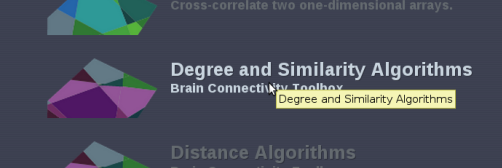
\includegraphics[width=\linewidth]{Handout_UI_ModellingStructuralLesions_Analysis}%
  \caption{Compute network metrics}%
  \label{fig:step_01}%
\end{figure}

%%%%%%%%%%%%%%%%%%%%%%%%%% STEPS %%%%%%%%%%%%%%%%%%%%%%%%%%%%%%%%%%%%%
\begin{formal}
  \begin{enumerate}
  \item Select degree and similarity algorithms. 
  \item Select the metric you want to compute and the connectivity matrix used as input. Click on launch. 
  \end{enumerate}
\end{formal}
%%%%%%%%%%%%%%%%%%%%%%%%%%%%%%%%%%%%%%%%%%%%%%%%%%%%%%%%%%%%%%%%%%%%%


\noindent By default the last action will take you back to the Operations dashboard.
Once the algorithm is finished, you can see the results in a 2D layout of the
head, which gives an idea of the network topology based on the node-wise
metrics.

%%%%%%%%%%%%%%%%%%%%%%%%%% STEPS %%%%%%%%%%%%%%%%%%%%%%%%%%%%%%%%%%%%%
\begin{formal}
  \begin{enumerate}[resume]
  \setcounter{enumi}{2}
  \item Click on 
\includegraphics[width=0.042\linewidth]{nodeConnectivityMeasure}. On
  the overlay window you can already see a summary of the basic descriptive
  statistics (Fig.~\ref{fig:step_02}).

  \item From the Visualizers tab launch the Topographic View.
  \end{enumerate}
\end{formal}
%%%%%%%%%%%%%%%%%%%%%%%%%%%%%%%%%%%%%%%%%%%%%%%%%%%%%%%%%%%%%%%%%%%%%

\begin{figure}[h]
  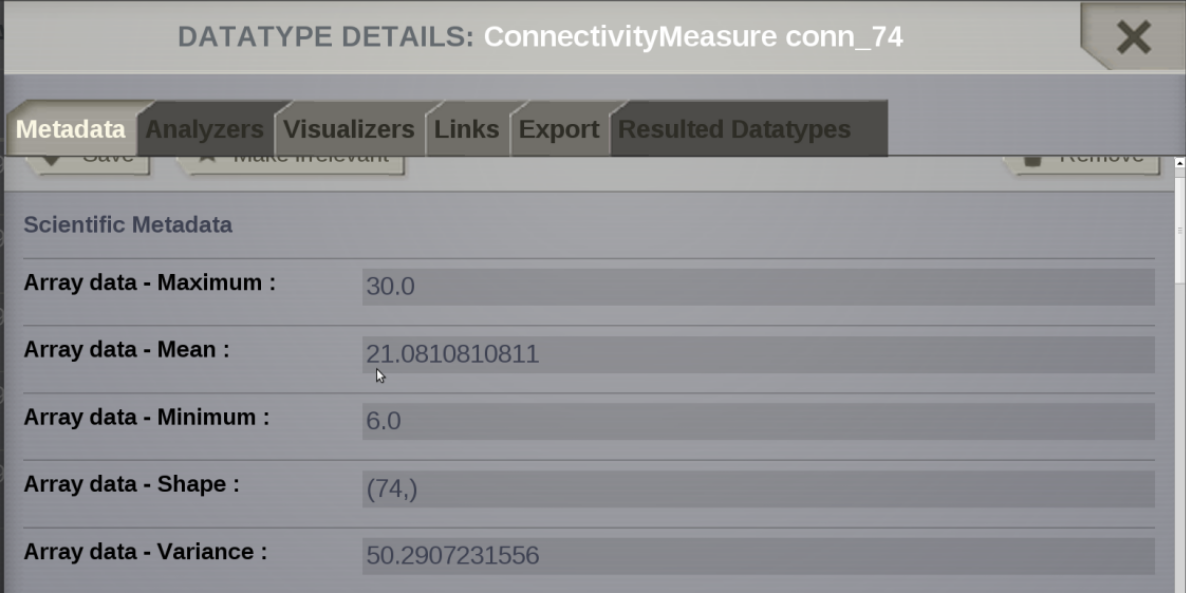
\includegraphics[width=\linewidth]{Handout_UI_ModellingStructuralLesions_AnalysisResult}%
  \caption{Descriptive summary}%
  \label{fig:step_02}%
\end{figure}

%%%%%%%%%%%%%%%%%%%%%%%%%% STEPS %%%%%%%%%%%%%%%%%%%%%%%%%%%%%%%%%%%%%
\noindent Other network measures were previously computed so we can also have a look at them. 
\begin{formal}
  \begin{enumerate}[resume] %% doesnt work with the formal enviornment :/
  \setcounter{enumi}{4}
  \item Select strength and clustering coefficient from the brain menu (Fig. ~\ref{fig:step_05}). Click on "Update Visualizer"
  \end{enumerate}
\end{formal}
%%%%%%%%%%%%%%%%%%%%%%%%%%%%%%%%%%%%%%%%%%%%%%%%%%%%%%%%%%%%%%%%%%%%%
\noindent It is possible to view and compare up to three metrics (Fig. ~\ref{fig:step_05b}).
\begin{figure}[h]
  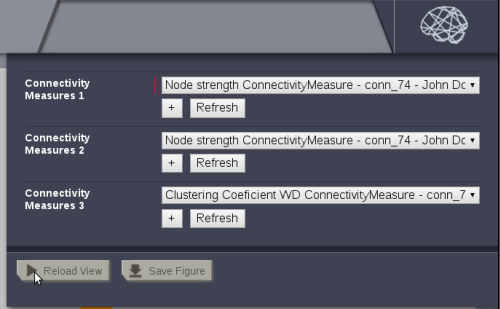
\includegraphics[width=0.5\linewidth]{Handout_UI_ModellingStructuralLesions_AnalysisView}%
  \caption{Select additional network metrics}%
  \label{fig:step_05}%
\end{figure}

\begin{figure}[h]
  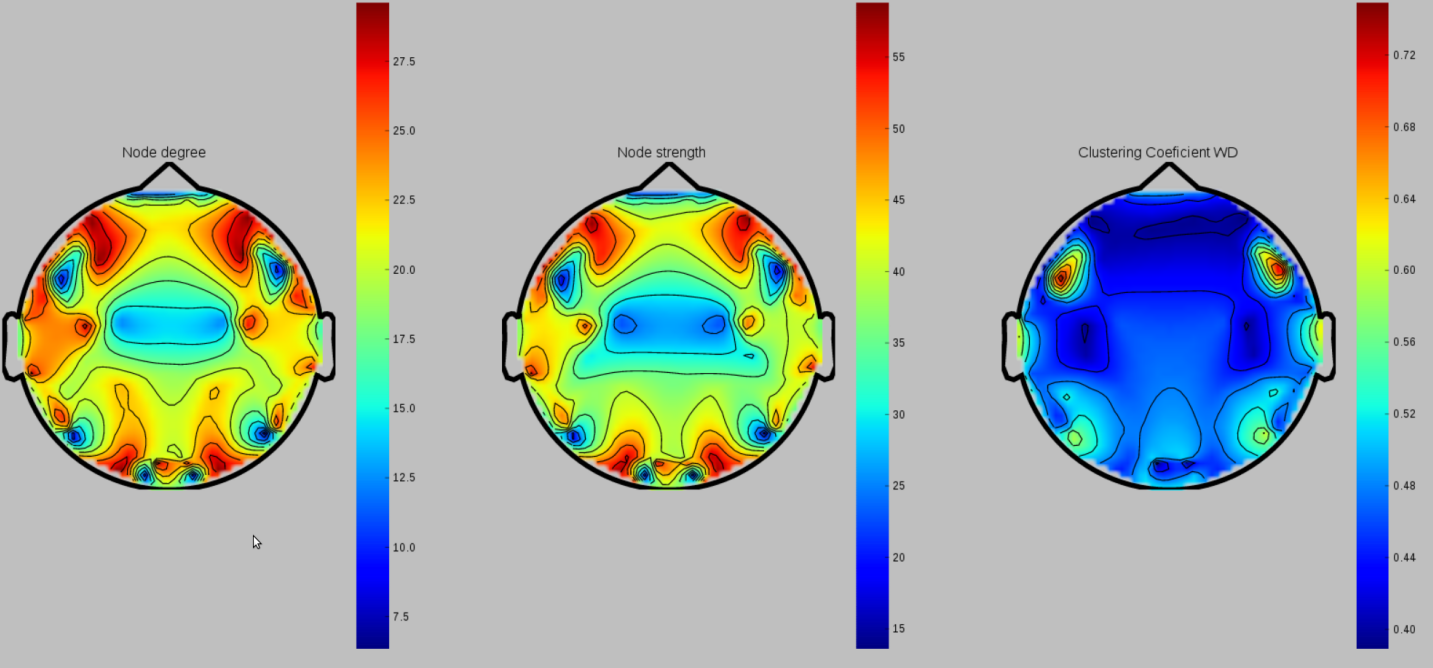
\includegraphics[width=0.9\linewidth]{Handout_UI_ModellingStructuralLesions_AnalysisResultCompare}%
  \caption{View and compare network metrics}%
  \label{fig:step_05b}%
\end{figure}
\newpage
\subsection{Steps: Interacting with the Connectome}

\noindent Figure~\ref{fig:fig} shows the connectivity editor. To get there, go to the
\textsc{Connectivity} area $\rightarrow$ \textsc{Large scale}. Several
displays are available for the matrices and some of them may use the node-wise
metrics to set the colour and size of the nodes. If you do not select any
metric before launching the connectivity editor, you can always set these
properties later.
\begin{figure}[h]
  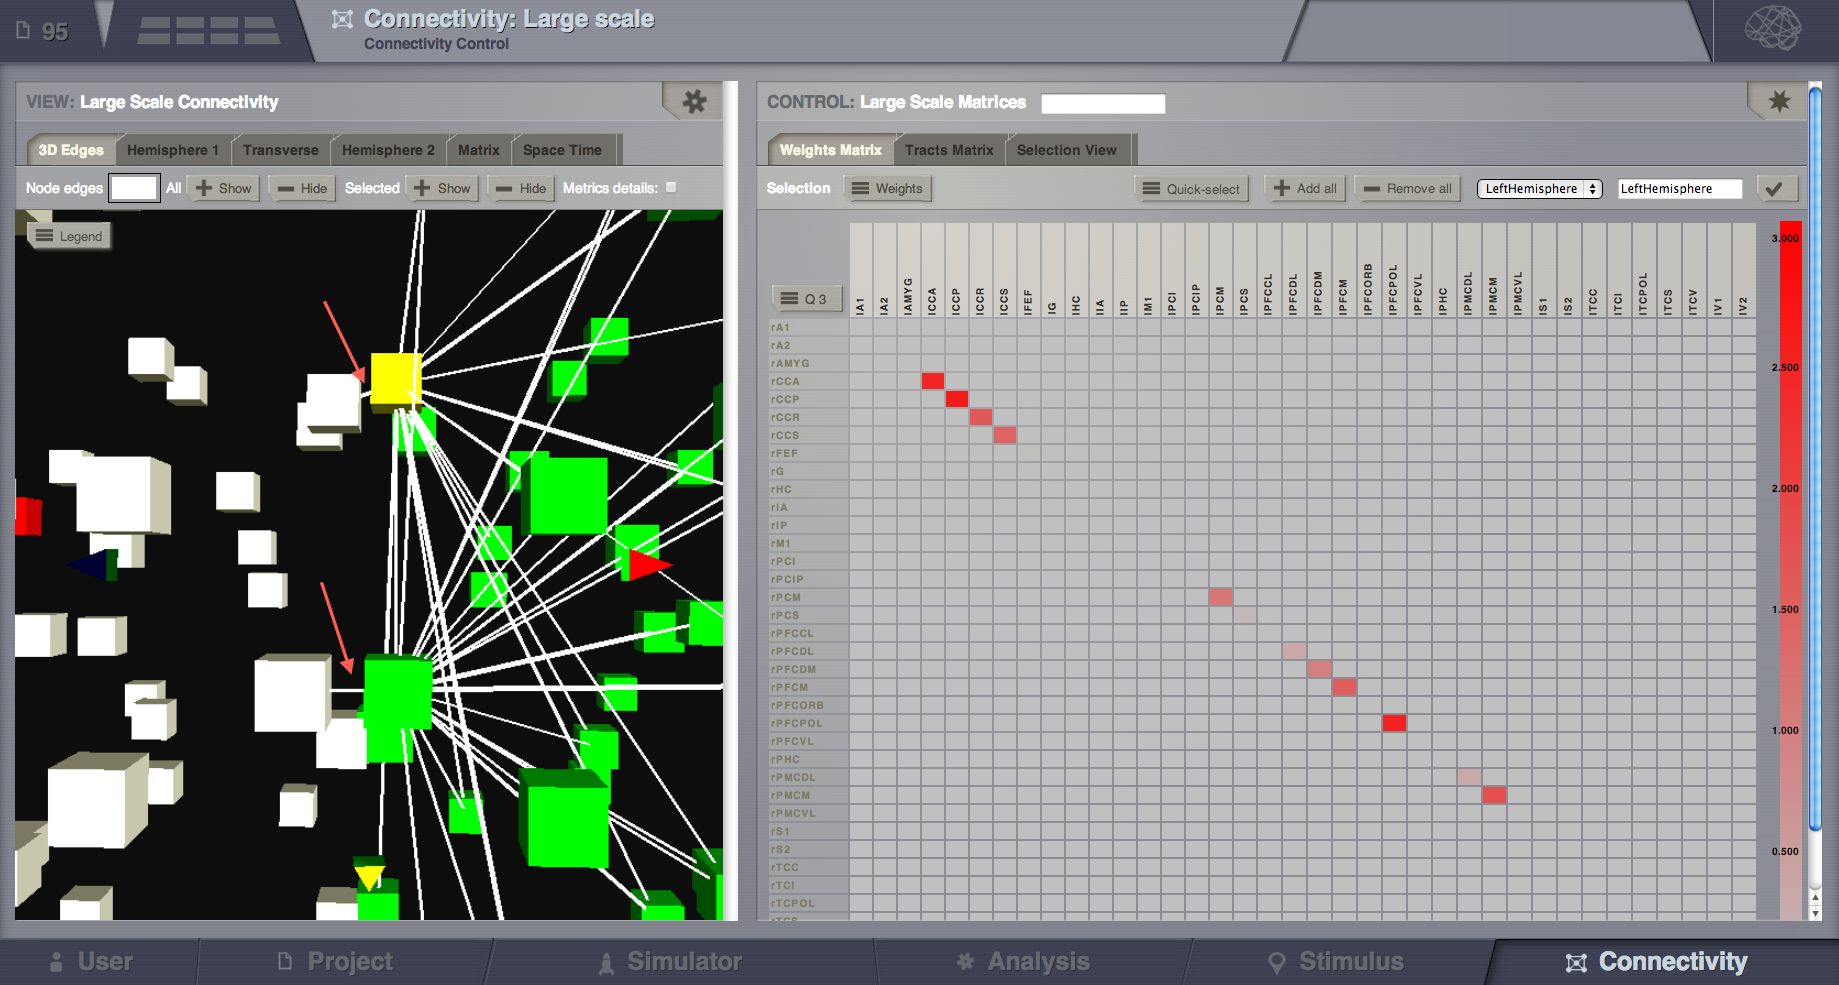
\includegraphics[width=\linewidth]{steps_Connectivity_ShowConnections.png}%
  \caption{Long-range connectivity editor}%
  \label{fig:fig}%
\end{figure}

\noindent Sometimes you may need to modify the connectivity, for instance, by deleting
specific nodes or edges. As working examples we will remove the subcortical
nuclei (nodes).
\begin{formal}
  \begin{enumerate}
  \setcounter{enumi}{5}
  \item In the quick-select menu remove the labels corresponding to these regions. Apply the changes (Fig.~\ref{fig:step_06}). 
  \item Save the node selection. This list can be used in other areas as well.
  \end{enumerate}
\end{formal}

\begin{figure}%
  \fbox{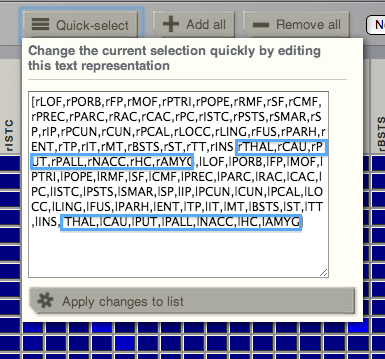
\includegraphics[width=0.82\linewidth]{Handout_UI_ModellingStructuralLesions_RemoveThalamicNodes.png}}\\
  \fbox{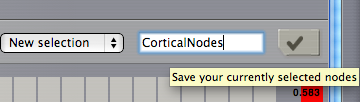
\includegraphics[width=0.82\linewidth]{Handout_UI_ModellingStructuralLesions_SaveSelection}}\\
  \fbox{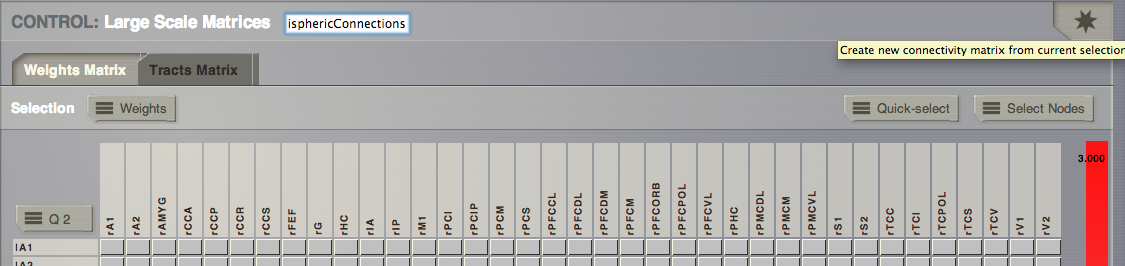
\includegraphics[width=0.82\linewidth]{Handout_UI_ModellingStructuralLesions_SaveNewMatrix}}\\
  \fbox{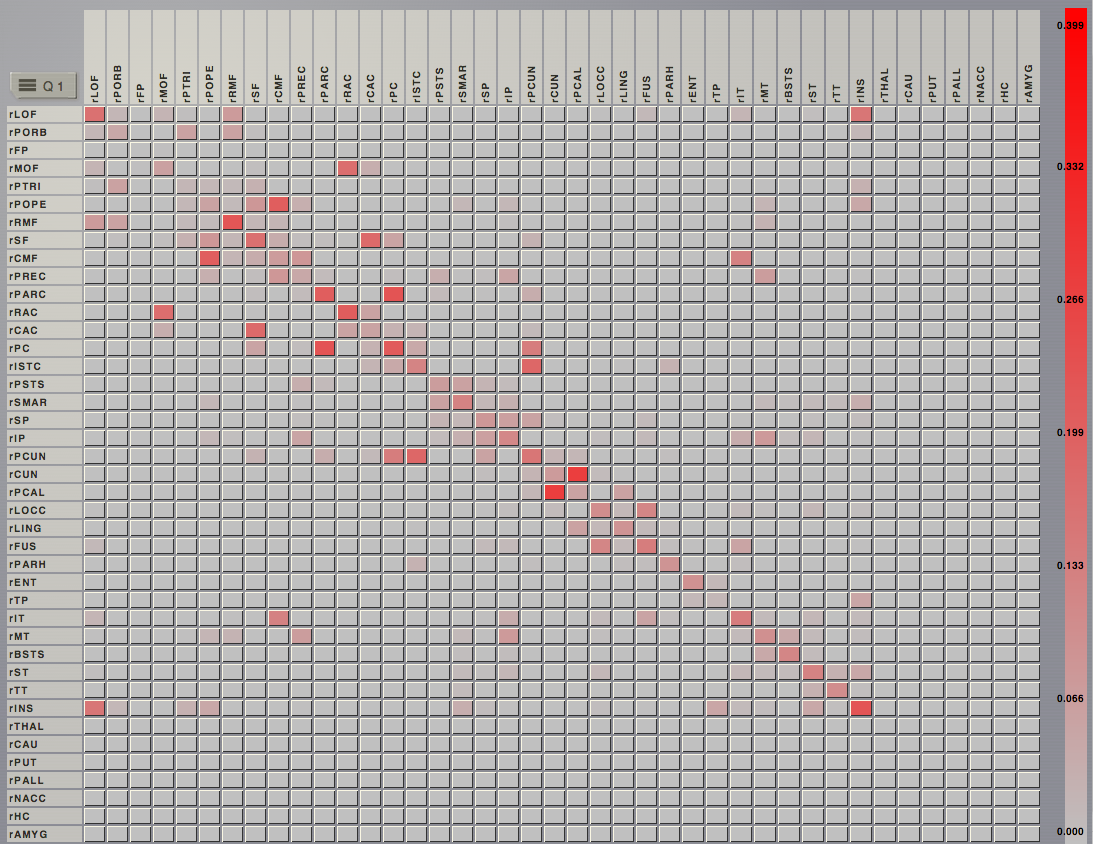
\includegraphics[width=0.82\linewidth]{Handout_UI_ModellingStructuralLesions_NewMatrix}}
  \caption{Edit and save node selection. Save the matrix as a new Connectivity. The connections of the inactive nodes were removed.}
  \label{fig:step_06}
\end{figure}
%TODO: add tables with region labels once we agree on the dataset will be using for this tutorial
 
\noindent In the connectivity editor the nodes that are not in the selection appear as if they were switched 'off'. 
You can save the new connectivity matrix, where the connections comprising the inactive nodes will be set to zero (so they are effectively removed). 

TODO: there is much more that we can include here. Some steps will be redundant with the tutorials and documentation.


\subsection{Steps: Simulation}

\noindent we can now evaluate the difference between the activity generated by both Connectomes. 
Go to the \textsc{simulator} area.

\begin{formal}
  \begin{enumerate}
  \setcounter{enumi}{7}
  \item Set up the brain network model according to the parameters in Table X. (This will be already available, but people can do it anyway).
  \item Launch the simulation.
  \item BOLD signals are already available.
  \end{enumerate}
\end{formal}

\section{Results}\label{sec:results}
If the time-series were processed in matlab or python to obtain certain
figures like Fig.~\ref{fig:fig_results}, then they should be reproducible.
Provide a code snippet to reproduce the figure. Add some conclusions.

\begin{figure}[h]
  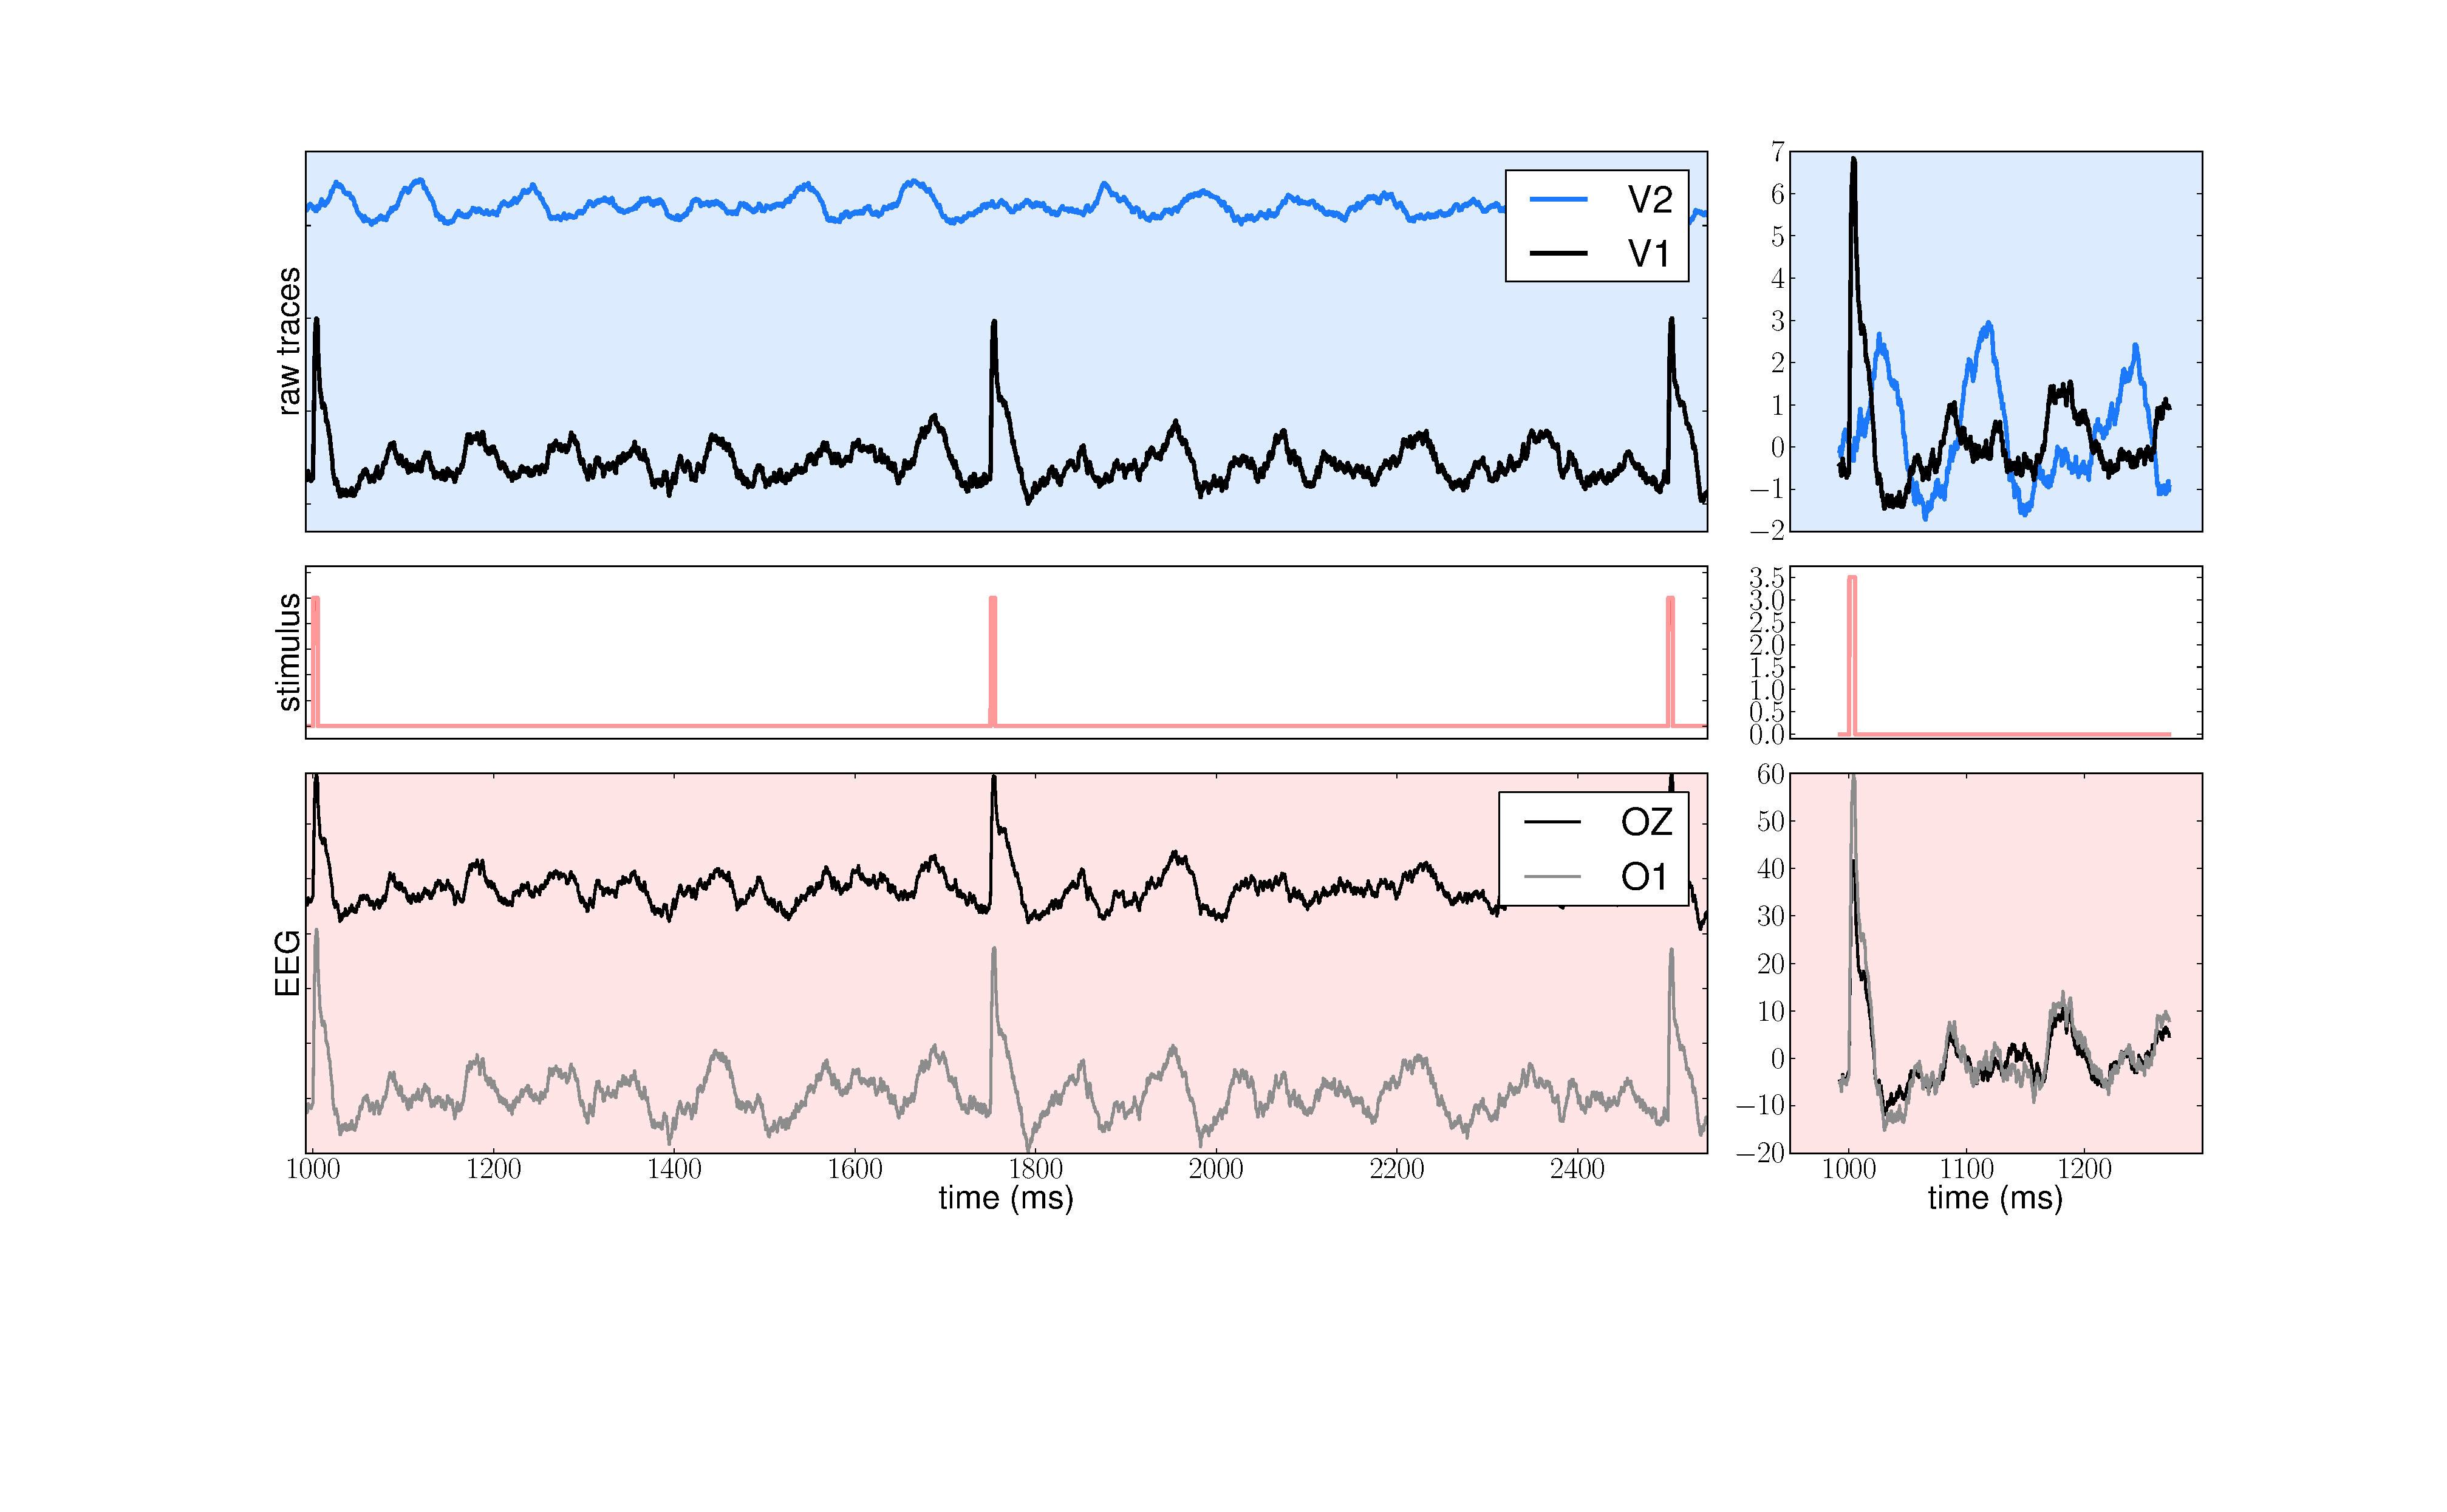
\includegraphics[width=\linewidth]{results_Example_ER_stochastic.pdf}%
  \caption{Long-range connectivity editor}%
  \label{fig:fig_results}%
\end{figure}


\section{More Documentation}\label{sec:more-doc}
For more documentation on The Virtual Brain, please see the following articles \cite{Sanz-Leon_2013, Spiegler_2013, Woodman_2014, Jirsa_2010b}


\section{Support}\label{sec:support}

The official TVB webiste is \url{www.thevirtualbrain.org}.  
All the documentation and tutorials are hosted on \url{the-virtual-brain.github.io}.
You'll find our public \smallcaps{git} repository at \url{https://github.com/the-virtual-brain}. 
For questions and bug reports we have a users group \url{https://groups.google.com/forum/#!forum/tvb-users}

\bibliography{tvb_references}
\bibliographystyle{plainnat}

\end{document}